% ============================================================================
% Digital Finance for Supervision - Program Handout
% MSCA DIGITAL Network Workshop at the European Central Bank
% December 3, 2026
% ============================================================================
\documentclass[a4paper,10pt]{article}

% --- Packages ---
\usepackage[top=12mm, bottom=14mm, left=14mm, right=14mm]{geometry}
\usepackage[T1]{fontenc}
\usepackage[utf8]{inputenc}
\usepackage{helvet}
\renewcommand{\familydefault}{\sfdefault}
\usepackage[table,dvipsnames]{xcolor}
\usepackage{tikz}
\usetikzlibrary{calc,positioning}
\usepackage{tabularx}
\usepackage{booktabs}
\usepackage{enumitem}
\usepackage[hidelinks]{hyperref}
\usepackage{qrcode}
\usepackage{fontawesome5}
\usepackage{microtype}
\usepackage{parskip}
\usepackage{multicol}

% --- Colors ---
\definecolor{ecbblue}{HTML}{003399}
\definecolor{ecbgold}{HTML}{FFD700}
\definecolor{digitalblue}{HTML}{2E5090}
\definecolor{darkbg}{HTML}{1a1a2e}
\definecolor{lightbg}{HTML}{F0F0F0}
\definecolor{lightblue}{HTML}{E8EEF7}
\definecolor{lightgold}{HTML}{FFF8DC}
\definecolor{medgray}{HTML}{666666}
\definecolor{breakgray}{HTML}{E8E8E8}
\definecolor{sessionblue}{HTML}{DFEAF8}
\definecolor{keynotecolor}{HTML}{FFF3CD}

% --- No page numbers ---
\pagestyle{empty}

% --- Document ---
\begin{document}

% ============================================================================
% HEADER
% ============================================================================
\begin{tikzpicture}[remember picture, overlay]
  % Blue header bar
  \fill[ecbblue]
    ($(current page.north west)$) rectangle ($(current page.north east) + (0,-28mm)$);
  % Gold accent line
  \draw[ecbgold, line width=2pt]
    ($(current page.north west) + (0,-28mm)$) -- ($(current page.north east) + (0,-28mm)$);
  % Title text
  \node[anchor=west, text=white] at ($(current page.north west) + (16mm,-10mm)$)
    {\fontsize{18}{20}\selectfont\bfseries Digital Finance for Supervision};
  \node[anchor=west, text=ecbgold] at ($(current page.north west) + (16mm,-18mm)$)
    {\fontsize{10}{12}\selectfont MSCA DIGITAL Network Workshop at the European Central Bank};
  % Date and venue on right
  \node[anchor=east, text=white, align=right] at ($(current page.north east) + (-16mm,-10mm)$)
    {\fontsize{10}{12}\selectfont\bfseries Thursday, December 3, 2026};
  \node[anchor=east, text=ecbgold, align=right] at ($(current page.north east) + (-16mm,-18mm)$)
    {\fontsize{9}{11}\selectfont Sonnemannstrasse 20, 60314 Frankfurt am Main};
  % Thin gold line under subtitle
  \draw[ecbgold, line width=0.5pt, opacity=0.5]
    ($(current page.north west) + (16mm,-23mm)$) -- ($(current page.north east) + (-16mm,-23mm)$);
\end{tikzpicture}

\vspace{22mm}

% ============================================================================
% PROGRAM TITLE
% ============================================================================
\begin{center}
  {\Large\bfseries\color{ecbblue} Workshop Program}\\[2pt]
  {\color{ecbgold}\rule{4cm}{1.5pt}}
\end{center}

\vspace{4mm}

% ============================================================================
% SCHEDULE TABLE
% ============================================================================
\renewcommand{\arraystretch}{1.0}
\setlength{\tabcolsep}{0pt}

\begin{tabularx}{\textwidth}{%
  >{\raggedright\arraybackslash\bfseries\color{ecbblue}}p{28mm}%
  >{\raggedright\arraybackslash}p{44mm}%
  X%
}

% --- Morning Header ---
\multicolumn{3}{l}{%
  \cellcolor{ecbblue}\hspace{3mm}%
  \raisebox{2pt}{\color{white}\bfseries\normalsize MORNING SESSION}%
  \hspace{\fill}%
}\\[1pt]

% Registration
\rowcolor{breakgray}
\hspace{3mm}10:00\,--\,10:15 &
\hspace{2mm}\textbf{Registration} &
\hspace{2mm}{\small Welcome coffee and badge collection} \\[1pt]

% Opening Remarks
\rowcolor{white}
\hspace{3mm}10:15\,--\,10:30 &
\hspace{2mm}\textbf{Opening Remarks} &
\hspace{2mm}{\small Welcome by ECB hosts and DIGITAL network coordinator. Introduction to the workshop themes and objectives.} \\[1pt]

% Keynote 1
\rowcolor{keynotecolor}
\hspace{3mm}10:30\,--\,11:15 &
\hspace{2mm}\textbf{Keynote Address 1} &
\hspace{2mm}{\small\color{ecbblue}\bfseries Speaker: TBA}\newline
\hspace{2mm}{\small AI and the future of banking supervision.}\newline
\hspace{2mm}{\footnotesize\color{medgray}\faIcon{star}~Keynote $\cdot$ 45 minutes including Q\&A} \\[1pt]

% Research Session 1
\rowcolor{sessionblue}
\hspace{3mm}11:15\,--\,12:00 &
\hspace{2mm}\textbf{Research Session 1} &
\hspace{2mm}{\small\color{ecbblue}\bfseries AI/ML for Bank Supervision}\newline
\hspace{2mm}{\small Three research presentations (15 min each) on machine learning}\newline
\hspace{2mm}{\small applications for supervisory risk assessment and early warning.}\newline
\hspace{2mm}{\footnotesize\color{medgray}\faIcon{microphone-alt}~Talk 1 $\cdot$ Talk 2 $\cdot$ Talk 3 --- Speakers TBA} \\[1pt]

% Lunch
\rowcolor{breakgray}
\hspace{3mm}12:00\,--\,13:00 &
\hspace{2mm}\textbf{Lunch \& Networking} &
\hspace{2mm}{\small Buffet lunch provided for all participants. Opportunity for}\newline
\hspace{2mm}{\small informal discussions and networking with speakers and peers.} \\[1pt]

% --- Afternoon Header ---
\multicolumn{3}{l}{%
  \cellcolor{ecbblue}\hspace{3mm}%
  \raisebox{2pt}{\color{white}\bfseries\normalsize AFTERNOON SESSION}%
  \hspace{\fill}%
}\\[1pt]

% Keynote 2 / Panel
\rowcolor{keynotecolor}
\hspace{3mm}13:00\,--\,13:45 &
\hspace{2mm}\textbf{Keynote 2 / Panel} &
\hspace{2mm}{\small\color{ecbblue}\bfseries LLMs in Supervision --- Speaker(s): TBA}\newline
\hspace{2mm}{\small Expert perspectives on how large language models are transforming}\newline
\hspace{2mm}{\small supervisory processes, with practical demonstrations and discussion.}\newline
\hspace{2mm}{\footnotesize\color{medgray}\faIcon{star}~Keynote / Panel $\cdot$ 45 minutes including Q\&A} \\[1pt]

% Research Session 2
\rowcolor{sessionblue}
\hspace{3mm}13:45\,--\,14:30 &
\hspace{2mm}\textbf{Research Session 2} &
\hspace{2mm}{\small\color{ecbblue}\bfseries NLP \& SupTech Applications}\newline
\hspace{2mm}{\small Three research presentations (15 min each) on NLP techniques}\newline
\hspace{2mm}{\small for regulatory reporting, compliance, and supervisory intelligence.}\newline
\hspace{2mm}{\footnotesize\color{medgray}\faIcon{microphone-alt}~Talk 4 $\cdot$ Talk 5 $\cdot$ Talk 6 --- Speakers TBA} \\[1pt]

% Panel Discussion
\rowcolor{keynotecolor!60}
\hspace{3mm}14:30\,--\,14:50 &
\hspace{2mm}\textbf{Panel Discussion} &
\hspace{2mm}{\small\color{ecbblue}\bfseries The Future of Digital Supervision}\newline
\hspace{2mm}{\small Moderated discussion with keynote speakers and senior ECB staff on}\newline
\hspace{2mm}{\small the roadmap for SupTech adoption and research priorities.} \\[1pt]

% Closing Remarks
\rowcolor{white}
\hspace{3mm}14:50\,--\,15:00 &
\hspace{2mm}\textbf{Closing Remarks} &
\hspace{2mm}{\small Summary of key takeaways, outlook for future collaboration, and}\newline
\hspace{2mm}{\small closing words by workshop co-chairs.} \\[1pt]

\end{tabularx}
\renewcommand{\arraystretch}{1.0}

\vspace{5mm}

% ============================================================================
% LEGEND
% ============================================================================
\begin{center}

\begin{tikzpicture}
  \fill[keynotecolor] (0,0) rectangle (0.4,0.4);
  \node[anchor=west] at (0.5,0.2) {\small\color{medgray} Keynote / Panel};
  \fill[sessionblue] (3.8,0) rectangle (4.2,0.4);
  \node[anchor=west] at (4.3,0.2) {\small\color{medgray} Research Session};
  \fill[breakgray] (7.8,0) rectangle (8.2,0.4);
  \node[anchor=west] at (8.3,0.2) {\small\color{medgray} Break / Registration};
\end{tikzpicture}
\end{center}

\vspace{3mm}

% ============================================================================
% BOTTOM INFORMATION
% ============================================================================
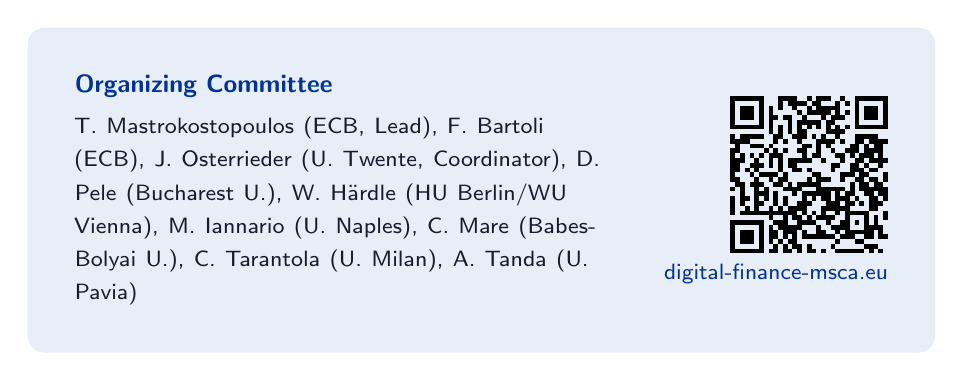
\begin{tikzpicture}
  \node[fill=lightblue, rounded corners=6pt, inner sep=6mm,
        text width=\textwidth-18mm, align=left] {%
    \begin{minipage}[c]{0.65\textwidth}
      {\small\bfseries\color{ecbblue} Organizing Committee}\\[3pt]
      {\footnotesize\color{darkbg}
      T.\ Mastrokostopoulos (ECB, Lead), F.\ Bartoli (ECB),
      J.\ Osterrieder (U.\ Twente, Coordinator),
      D.\ Pele (Bucharest U.), W.\ H\"ardle (HU Berlin/WU Vienna),
      M.\ Iannario (U.\ Naples), C.\ Mare (Babes-Bolyai U.),
      C.\ Tarantola (U.\ Milan), A.\ Tanda (U.\ Pavia)}
    \end{minipage}\hfill
    \begin{minipage}[c]{0.3\textwidth}
      \raggedleft
      \qrcode[height=2cm]{https://digital-finance-msca.eu/events/ecb-workshop-2026}\\[3pt]
      {\footnotesize\color{ecbblue}\url{digital-finance-msca.eu}}
    \end{minipage}
  };
\end{tikzpicture}

\vspace{3mm}

% Practical information row
\begin{multicols}{3}
  {\footnotesize
  \textbf{\color{ecbblue}\faIcon{wifi}\quad WiFi Access}\\
  Network: \textit{to be provided on-site}\\
  Password: \textit{see registration desk}
  }
\columnbreak
  {\footnotesize
  \textbf{\color{ecbblue}\faIcon{envelope}\quad Contact}\\
  info@digital-finance-msca.eu\\
  \url{https://digital-finance-msca.eu}
  }
\columnbreak
  {\footnotesize
  \textbf{\color{ecbblue}\faIcon{map-marker-alt}\quad Venue}\\
  European Central Bank\\
  Sonnemannstrasse 20, Frankfurt
  }
\end{multicols}

% ============================================================================
% FOOTER
% ============================================================================
\vfill

\begin{tikzpicture}[remember picture, overlay]
  % Gold line above footer
  \draw[ecbgold, line width=1pt]
    ($(current page.south west) + (14mm,20mm)$) -- ($(current page.south east) + (-14mm,20mm)$);
  % Funding text
  \node[anchor=south, text width=\textwidth-32mm, align=center]
    at ($(current page.south) + (0,8mm)$) {%
    {\scriptsize\color{medgray}
    Funded by the European Union's Horizon Europe programme under the Marie Sk\l{}odowska-Curie Grant Agreement No.\ 101119635
    (DIGITAL -- Digital Finance -- Reaching New Frontiers).
    Views and opinions expressed are those of the author(s) only and do not necessarily reflect those of the European Union or the European Research Executive Agency.}
  };
\end{tikzpicture}

\end{document}
